\documentclass{article}
\usepackage[utf8]{inputenc}
\usepackage[margin=0.70in]{geometry}
\usepackage{graphicx}

\title{HW 2-3: Parallelizing Particle Simulation Using CUDA and GPU}
\author{Andrew Chen, Xuan Jiang, Brian Park}
\date{March 2022}

\begin{document}

\maketitle

\section{Code}
\subsection{Data Structures}
\begin{itemize}
    \item \verb|bin_ids| \\
        This holds the head of the pointer of the next reference of the particle in the bin in \verb|particle_ids|.
    \item \verb|particle_ids| \\
        This is a mapping and reference of the particle ids. In it is stored \verb|len(bin_ids)| linked list, where each linked list contains the particle in that specific bin. The element inside \verb|particle_ids| will point to the next index of the particle. The end of the linked list or the null pointer is encoded as -1.
    
\end{itemize}

\subsection{Algorithm}
In general, compared to using prefix sum, this saves on memory allocation, but may seem to take a hit on spatial locality, since the linked list is not stored contiguously and cannot take advantage of the GPU cache. Another tradeoff that this design has is that it does not need to sort and can append to the linked list in $O(1)$ time using an atomic swap primitive in CUDA. Thus, the creation of the linked list can be called by a \verb|__global__| function, although the actual appending takes $O(n)$ time for each iteration per bin. But note that as the number of particles increase, the more bins that are created, so each bin will have a relatively small amount of particles, thus the $O(n)$ time mentioned earlier is smaller and latency of pointer chasing is essentially hidden to a smaller constant as you increase the number of particles. 

\subsection{Synchronization}
The only synchronization primitive that this code uses are atomic instructions \verb|atomicExch()| and \\ \verb|cudaDeviceSynchronize()|. We need \verb|atomicExch()| to append the linked list atomically and update the head of the head of the \verb|bin_ids| table of references. We need \verb|cudaDeviceSynchronize()| during every step of \verb|simulate_one_step| because we rebin the particles everytime after moving. To ensure that all the particles are in the right position before rebinning, we essentially put a barrier to ensure correctness of the particle's positions. Otherwise, the code may decide to bin particles without finishing moving.

\subsection{Other Design Choices}
Originally, we tried to use the GSI's recitation slides as a guide, using the prefix sum to compute the location of the \verb|particle_ids| into \verb|bin_ids| as the pointer to the location, since \verb|particles| would be sorted and stored contiguously into \verb|particle_ids|. But we had a lot of trouble figuring out how to make this ensure correctness, as in \verb|init_simulation| everything would seem correct, but after iterations in \verb|simulate_one_step|  there was synchronization issues where sometimes the bins wouldn't be sorted properly. Adding synchronization primitives such as \verb|cudaDeviceSynchronize()| and \verb|__syncthreads()| only slowed down the code and didn't fix correctness. Due to this weird correctness bug, we started from scratch again. We had the linked list implementation in mind, but were worried that pointer chasing would incur a lot of GPU cache misses. Given that the GPU architecture is very expensive and performant on registers and memory bandwidth, this type of concern should be free and very minimal. Given that the linked list implementation is under 4 seconds and pretty good compared to previous semester grades, we merged it into our main implementation. Ignoring correctness, the performance of prefix sum and sorting implementation was very bad, and it was probably due to the calls of \verb|cudaMemCpy| to do transfer data from CPU to GPU. Fortunately, the linked list implementation resides all of its computation on the GPU memory. Surprisingly, the code is very straightforward and cleaner than the original prefix sum and sorting implementation.

\subsection{Can We Do Better?}
If given enough time, abandoning the linked list implementation and redoing the prefix sum could give us better performance. But considering that a student on Piazza reached 1.5 seconds on 1 million particles (ours is around 1.56s), we considered this as our stopping point. To implement the prefix sum required more code and a lot more debugging, and it was frustrating to use \verb|cuda-gdb| as switching into GPU kernel threads was often confusing to understand. Instead, we printed statements by transferring copies to CPU for correctness.

\section{Performance}

\subsection{Log-Log Plot/Naive and our GPU implementation with linear behavior}
\centerline{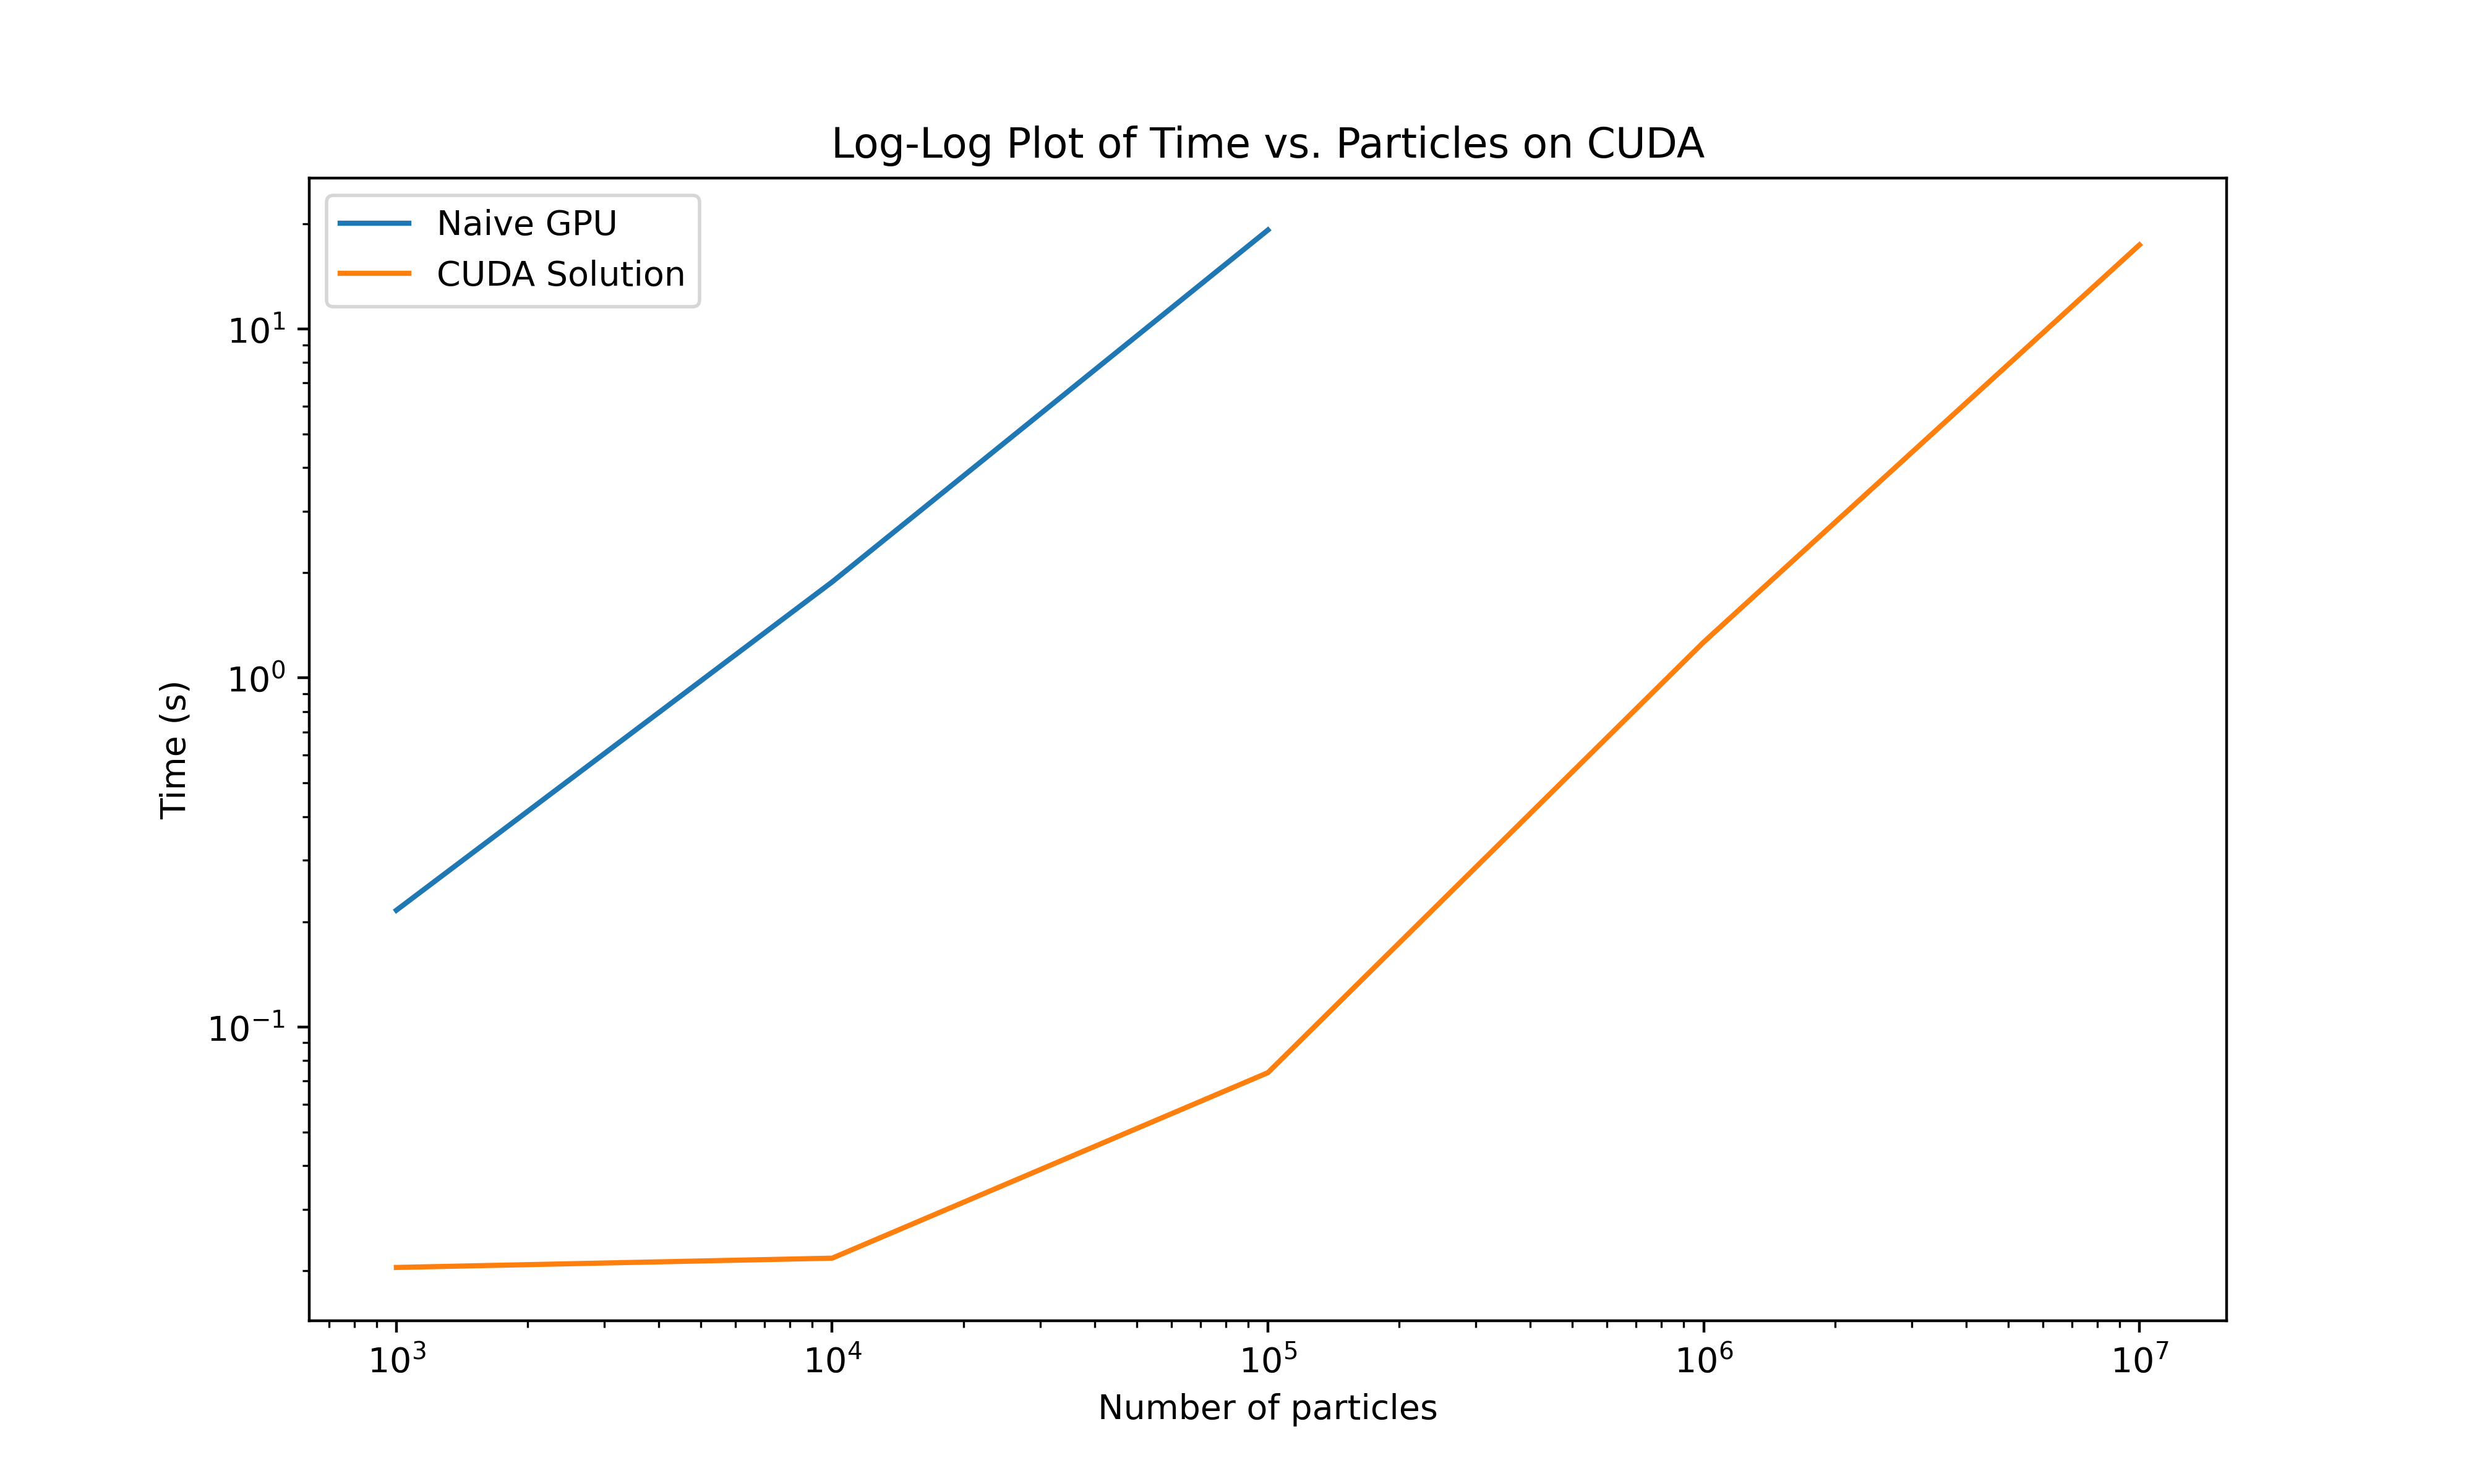
\includegraphics[width=6in]{figures/log-log.png}}

Above shows the plots of the GPU optimized performance compared to the naive implementation from the starter code. We a constant increase in performance for naive and our optimized solution is able to follow that increase but at a much lower time. This is essentially the Roofline model in effect, where we see our performance be in memory bound and change to compute bound at around $10^5$ particles.


\subsection{All Implmentations of HW 2 Compared}
\centerline{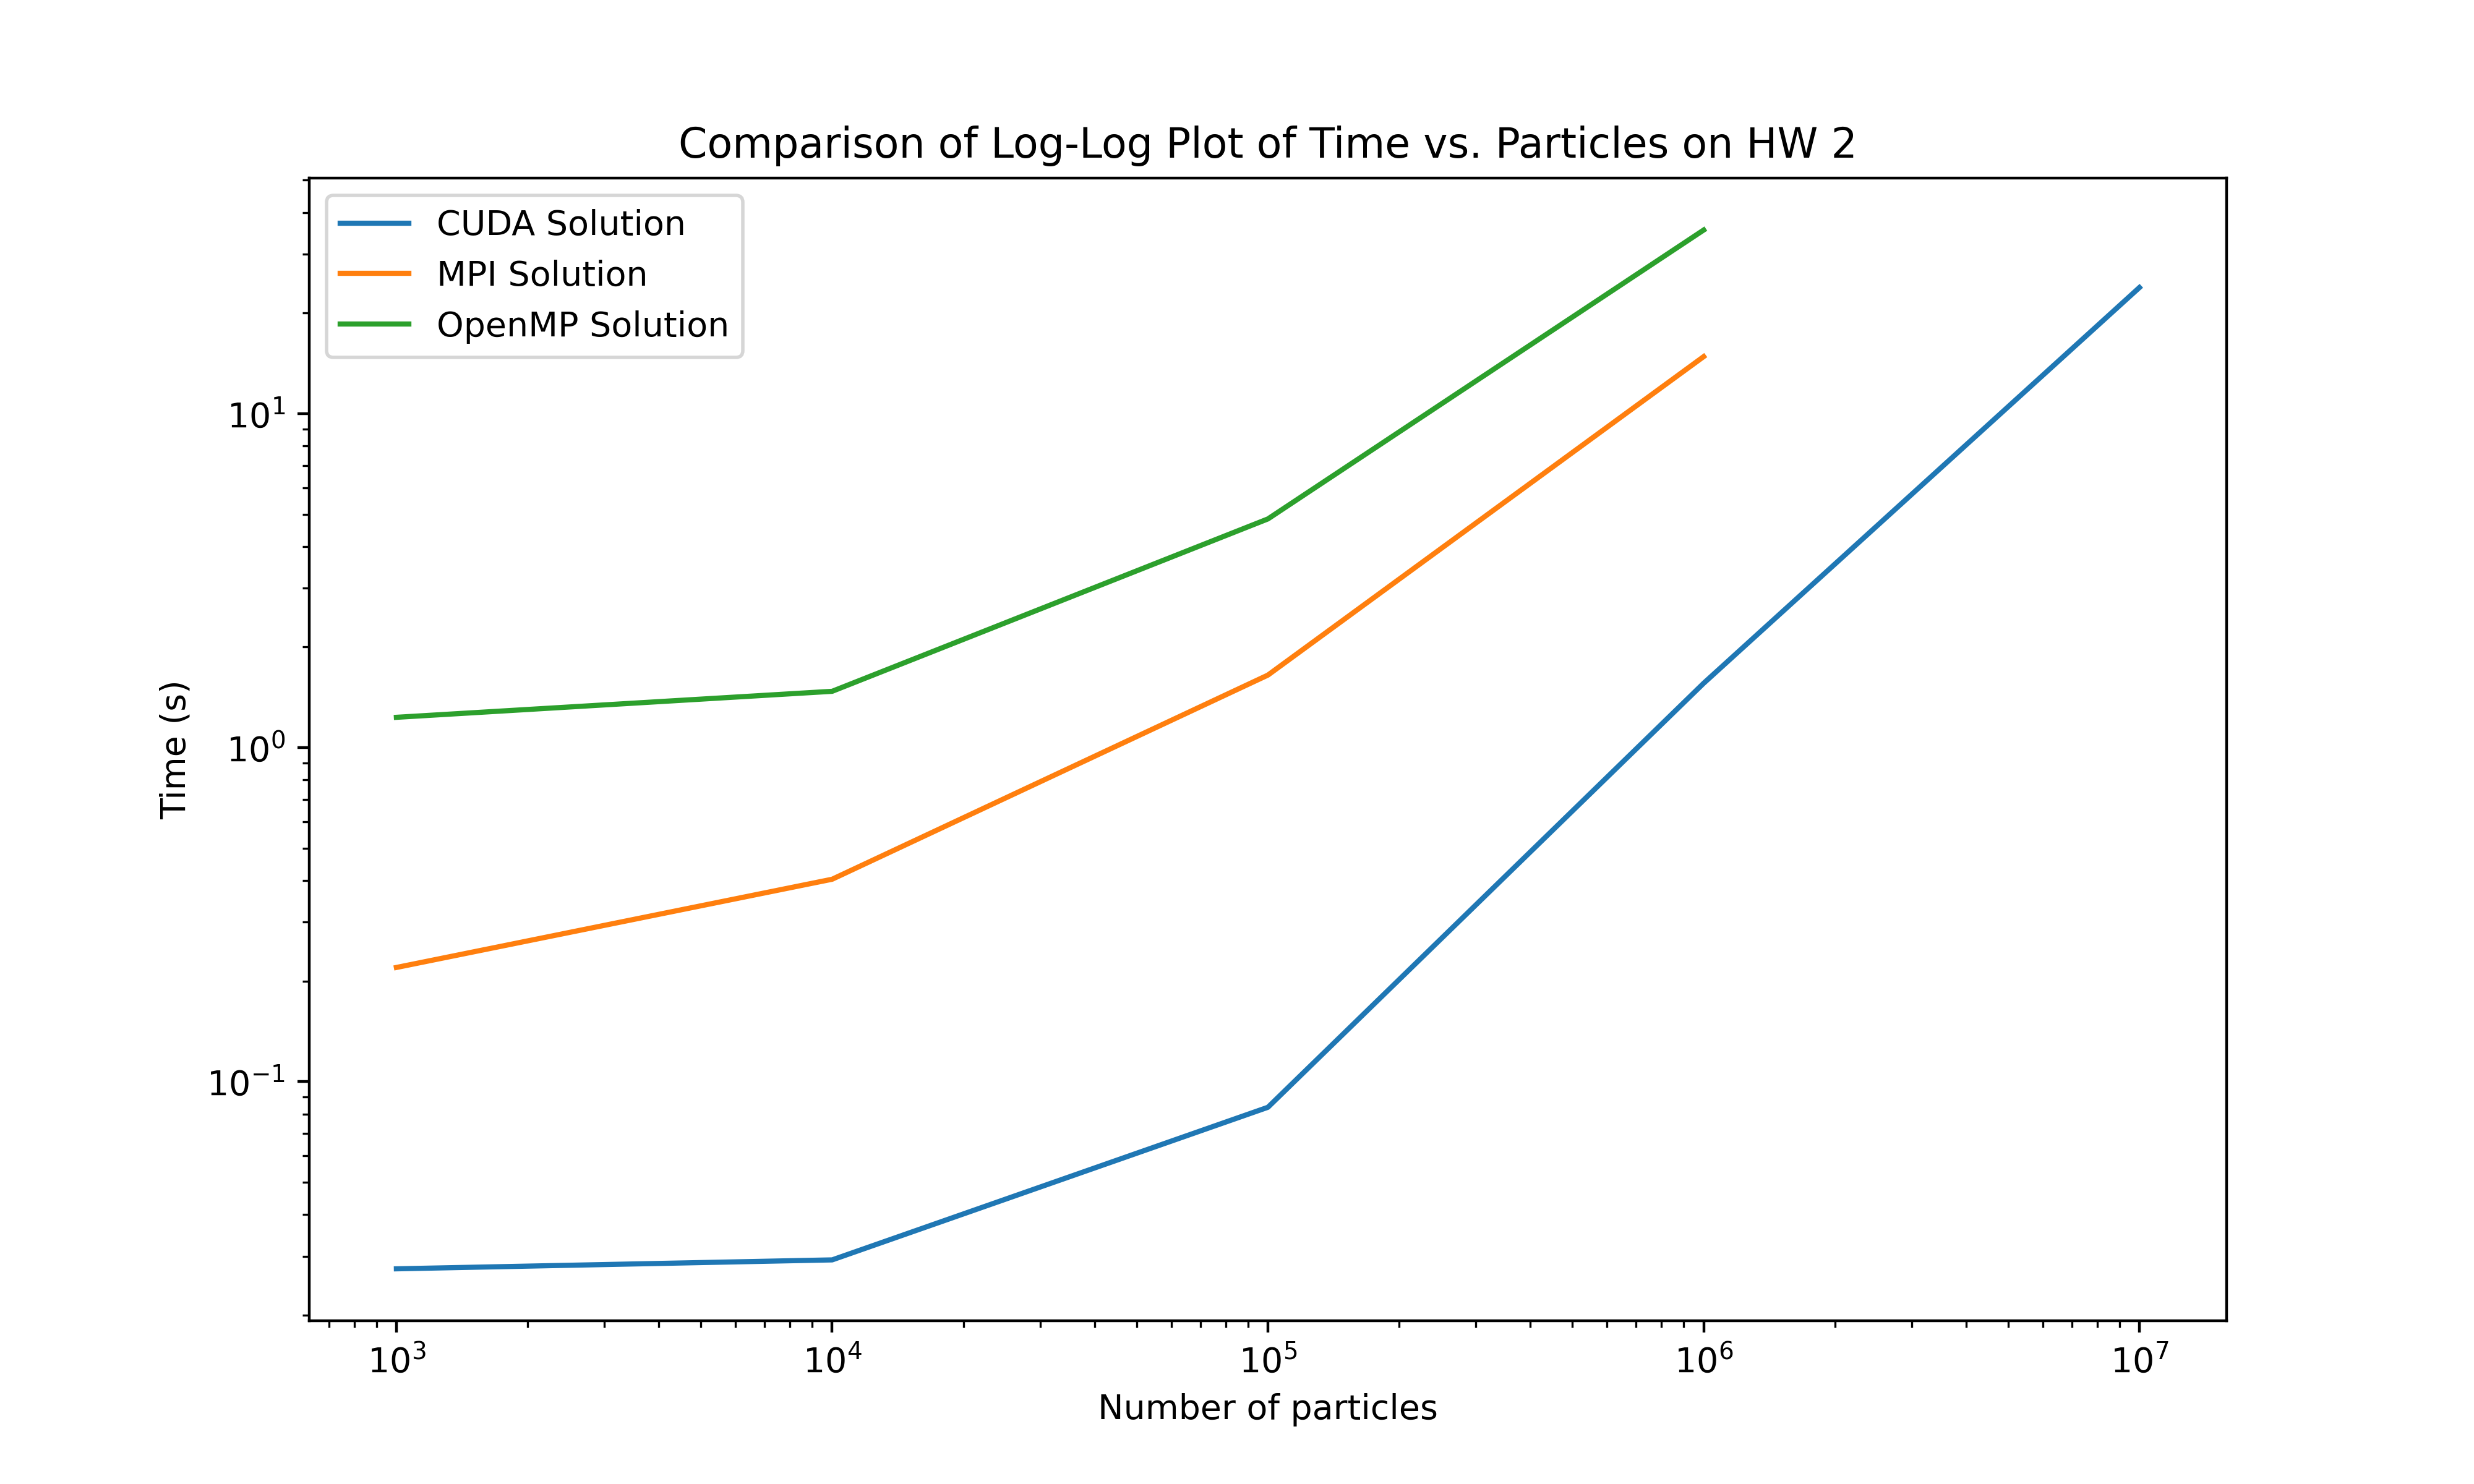
\includegraphics[width=6in]{figures/hw2-compare.png}}

Interestingly, we see all of our implementations from OpenMP, MPI, and CUDA graphed together. Amazingly, CUDA beats all of the implementation time wise. While benchmarking, we could not test 10 million particles on OpenMP and MPI as it would take too long. But even at 1 million particles, it's amazing to see how adding hardware improves speed by a lot. Notes that OpenMP was run on 68 threads on Cori, and MPI was run on 2 nodes with 68 processes (total 136 processes). Both were on Cori KNL nodes while CUDA was on bridges-2 node with 1 Nvidia Tesla V100 GPU (a whopping 5120 CUDA cores).

\subsection{Profiling}
Here is a dump of the profiling log from \verb|nvprof| for 1000 particles:

\begin{table}[]
\begin{tabular}{llllllll}
Type       & Time(\%) & Time     & Calls & Avg      & Min      & Max      & Name                   \\
GPU activities: &
  69.81\% &
  10.602ms &
  1000 &
  10.601us &
  5.4080us &
  11.872us &
  \begin{tabular}[c]{@{}l@{}}compute\_forces\_gpu\_bin\\ (particle\_t*, int, int, double, int*, int*)\end{tabular} \\
 &
  17.10\% &
  2.5970ms &
  1000 &
  2.5960us &
  2.5600us &
  2.8160us &
  move\_gpu(particle\_t*, int, double) \\
 &
  13.04\% &
  1.9810ms &
  1001 &
  1.9790us &
  1.9190us &
  9.6000us &
  \begin{tabular}[c]{@{}l@{}}binning(particle\_t*, \\ int, int, double, int*, int*)\end{tabular} \\
           & 0.04\%   & 6.7200us & 1     & 6.7200us & 6.7200us & 6.7200us & {[}CUDA memcpy HtoD{]} \\
API calls: & 86.51\%  & 208.47ms & 3     & 69.490ms & 2.9360us & 208.46ms & cudaMalloc             \\
           & 8.40\%   & 20.253ms & 2001  & 10.121us & 978ns    & 21.672us & cudaDeviceSynchronize  \\
           & 4.54\%   & 10.951ms & 3001  & 3.6490us & 3.2270us & 28.849us & cudaLaunchKernel       \\
           & 0.26\%   & 618.75us & 1     & 618.75us & 618.75us & 618.75us & cuDeviceTotalMem       \\
           & 0.23\%   & 565.39us & 101   & 5.5970us & 119ns    & 250.51us & cuDeviceGetAttribute   \\
           & 0.03\%   & 69.979us & 1     & 69.979us & 69.979us & 69.979us & cuDeviceGetName        \\
           & 0.02\%   & 39.924us & 1     & 39.924us & 39.924us & 39.924us & cudaMemcpy             \\
           & 0.00\%   & 7.6000us & 1     & 7.6000us & 7.6000us & 7.6000us & cudaFree               \\
           & 0.00\%   & 5.2530us & 1     & 5.2530us & 5.2530us & 5.2530us & cuDeviceGetPCIBusId    \\
           & 0.00\%   & 1.3850us & 3     & 461ns    & 218ns    & 925ns    & cuDeviceGetCount       \\
           & 0.00\%   & 1.0380us & 2     & 519ns    & 158ns    & 880ns    & cuDeviceGet            \\
           & 0.00\%   & 239ns    & 1     & 239ns    & 239ns    & 239ns    & cuDeviceGetUuid       
\end{tabular}
\end{table}

Unless profiling creates some overhead, we know that in general, it takes around 0.025 seconds or 25ms for 1000 particles. We see that 69\% of the GPU's time is spent on \verb|compute_forces_gpu|, which is obviously the bottleneck even on serial implementation. Surprisingly, not that much time is spend on \verb|move_gpu|, but the analysis is understandable as it doesn't do anything computationally expensive. And impressively, 
\verb|binning| takes 13\% of the GPU's time. It seems very fast to append to the linked list, and it's satisfying to know that pointer chasing doesn't seem to induce that much overhead or slowdown in performance given how binning works.

For fun, a dump of 1 million particles is shown below:

\begin{table}[]
\begin{tabular}{llllllll}
Type       & Time(\%) & Time     & Calls & Avg      & Min      & Max      & Name                                 \\
GPU activities: &
  61.73\% &
  959.97ms &
  1000 &
  959.97us &
  902.36us &
  1.1170ms &
  \begin{tabular}[c]{@{}l@{}}compute\_forces\_gpu\_bin(\\ particle\_t*, int, int, double, int*, int*)\end{tabular} \\
 &
  28.31\% &
  440.30ms &
  1001 &
  439.86us &
  387.42us &
  465.47us &
  \begin{tabular}[c]{@{}l@{}}binning(particle\_t*, int, \\ int, double, int*, int*)\end{tabular} \\
           & 9.26\%   & 143.95ms & 1000  & 143.95us & 139.23us & 149.85us & move\_gpu(particle\_t*, int, double) \\
           & 0.70\%   & 10.840ms & 1     & 10.840ms & 10.840ms & 10.840ms & {[}CUDA memcpy HtoD{]}               \\
API calls: & 86.73\%  & 1.54982s & 2001  & 774.52us & 940ns    & 1.4105ms & cudaDeviceSynchronize                \\
           & 11.91\%  & 212.88ms & 3     & 70.961ms & 230.32us & 212.32ms & cudaMalloc                           \\
           & 0.63\%   & 11.177ms & 3001  & 3.7240us & 3.2100us & 51.167us & cudaLaunchKernel                     \\
           & 0.62\%   & 11.050ms & 1     & 11.050ms & 11.050ms & 11.050ms & cudaMemcpy                           \\
           & 0.06\%   & 1.0764ms & 1     & 1.0764ms & 1.0764ms & 1.0764ms & cuDeviceTotalMem                     \\
           & 0.03\%   & 579.12us & 101   & 5.7330us & 124ns    & 260.01us & cuDeviceGetAttribute                 \\
           & 0.02\%   & 386.46us & 1     & 386.46us & 386.46us & 386.46us & cudaFree                             \\
           & 0.00\%   & 67.072us & 1     & 67.072us & 67.072us & 67.072us & cuDeviceGetName                      \\
           & 0.00\%   & 5.6740us & 1     & 5.6740us & 5.6740us & 5.6740us & cuDeviceGetPCIBusId                  \\
           & 0.00\%   & 1.2430us & 3     & 414ns    & 170ns    & 881ns    & cuDeviceGetCount                     \\
           & 0.00\%   & 885ns    & 2     & 442ns    & 127ns    & 758ns    & cuDeviceGet                          \\
           & 0.00\%   & 217ns    & 1     & 217ns    & 217ns    & 217ns    & cuDeviceGetUuid                     
\end{tabular}
\end{table}

Again, we see that with profiling, the scaling of particles scales well with the simulation. There are small shifts in percentages, such as binning and computing forces, but that is probably mainly due to the ratio between particles and bins and the number of times it can map to GPU kernels threads. At some point, binning takes more execution time then move for a certain number of particles. 

Here are more visuals to depict the profiling of GPU execution: \\

\centerline{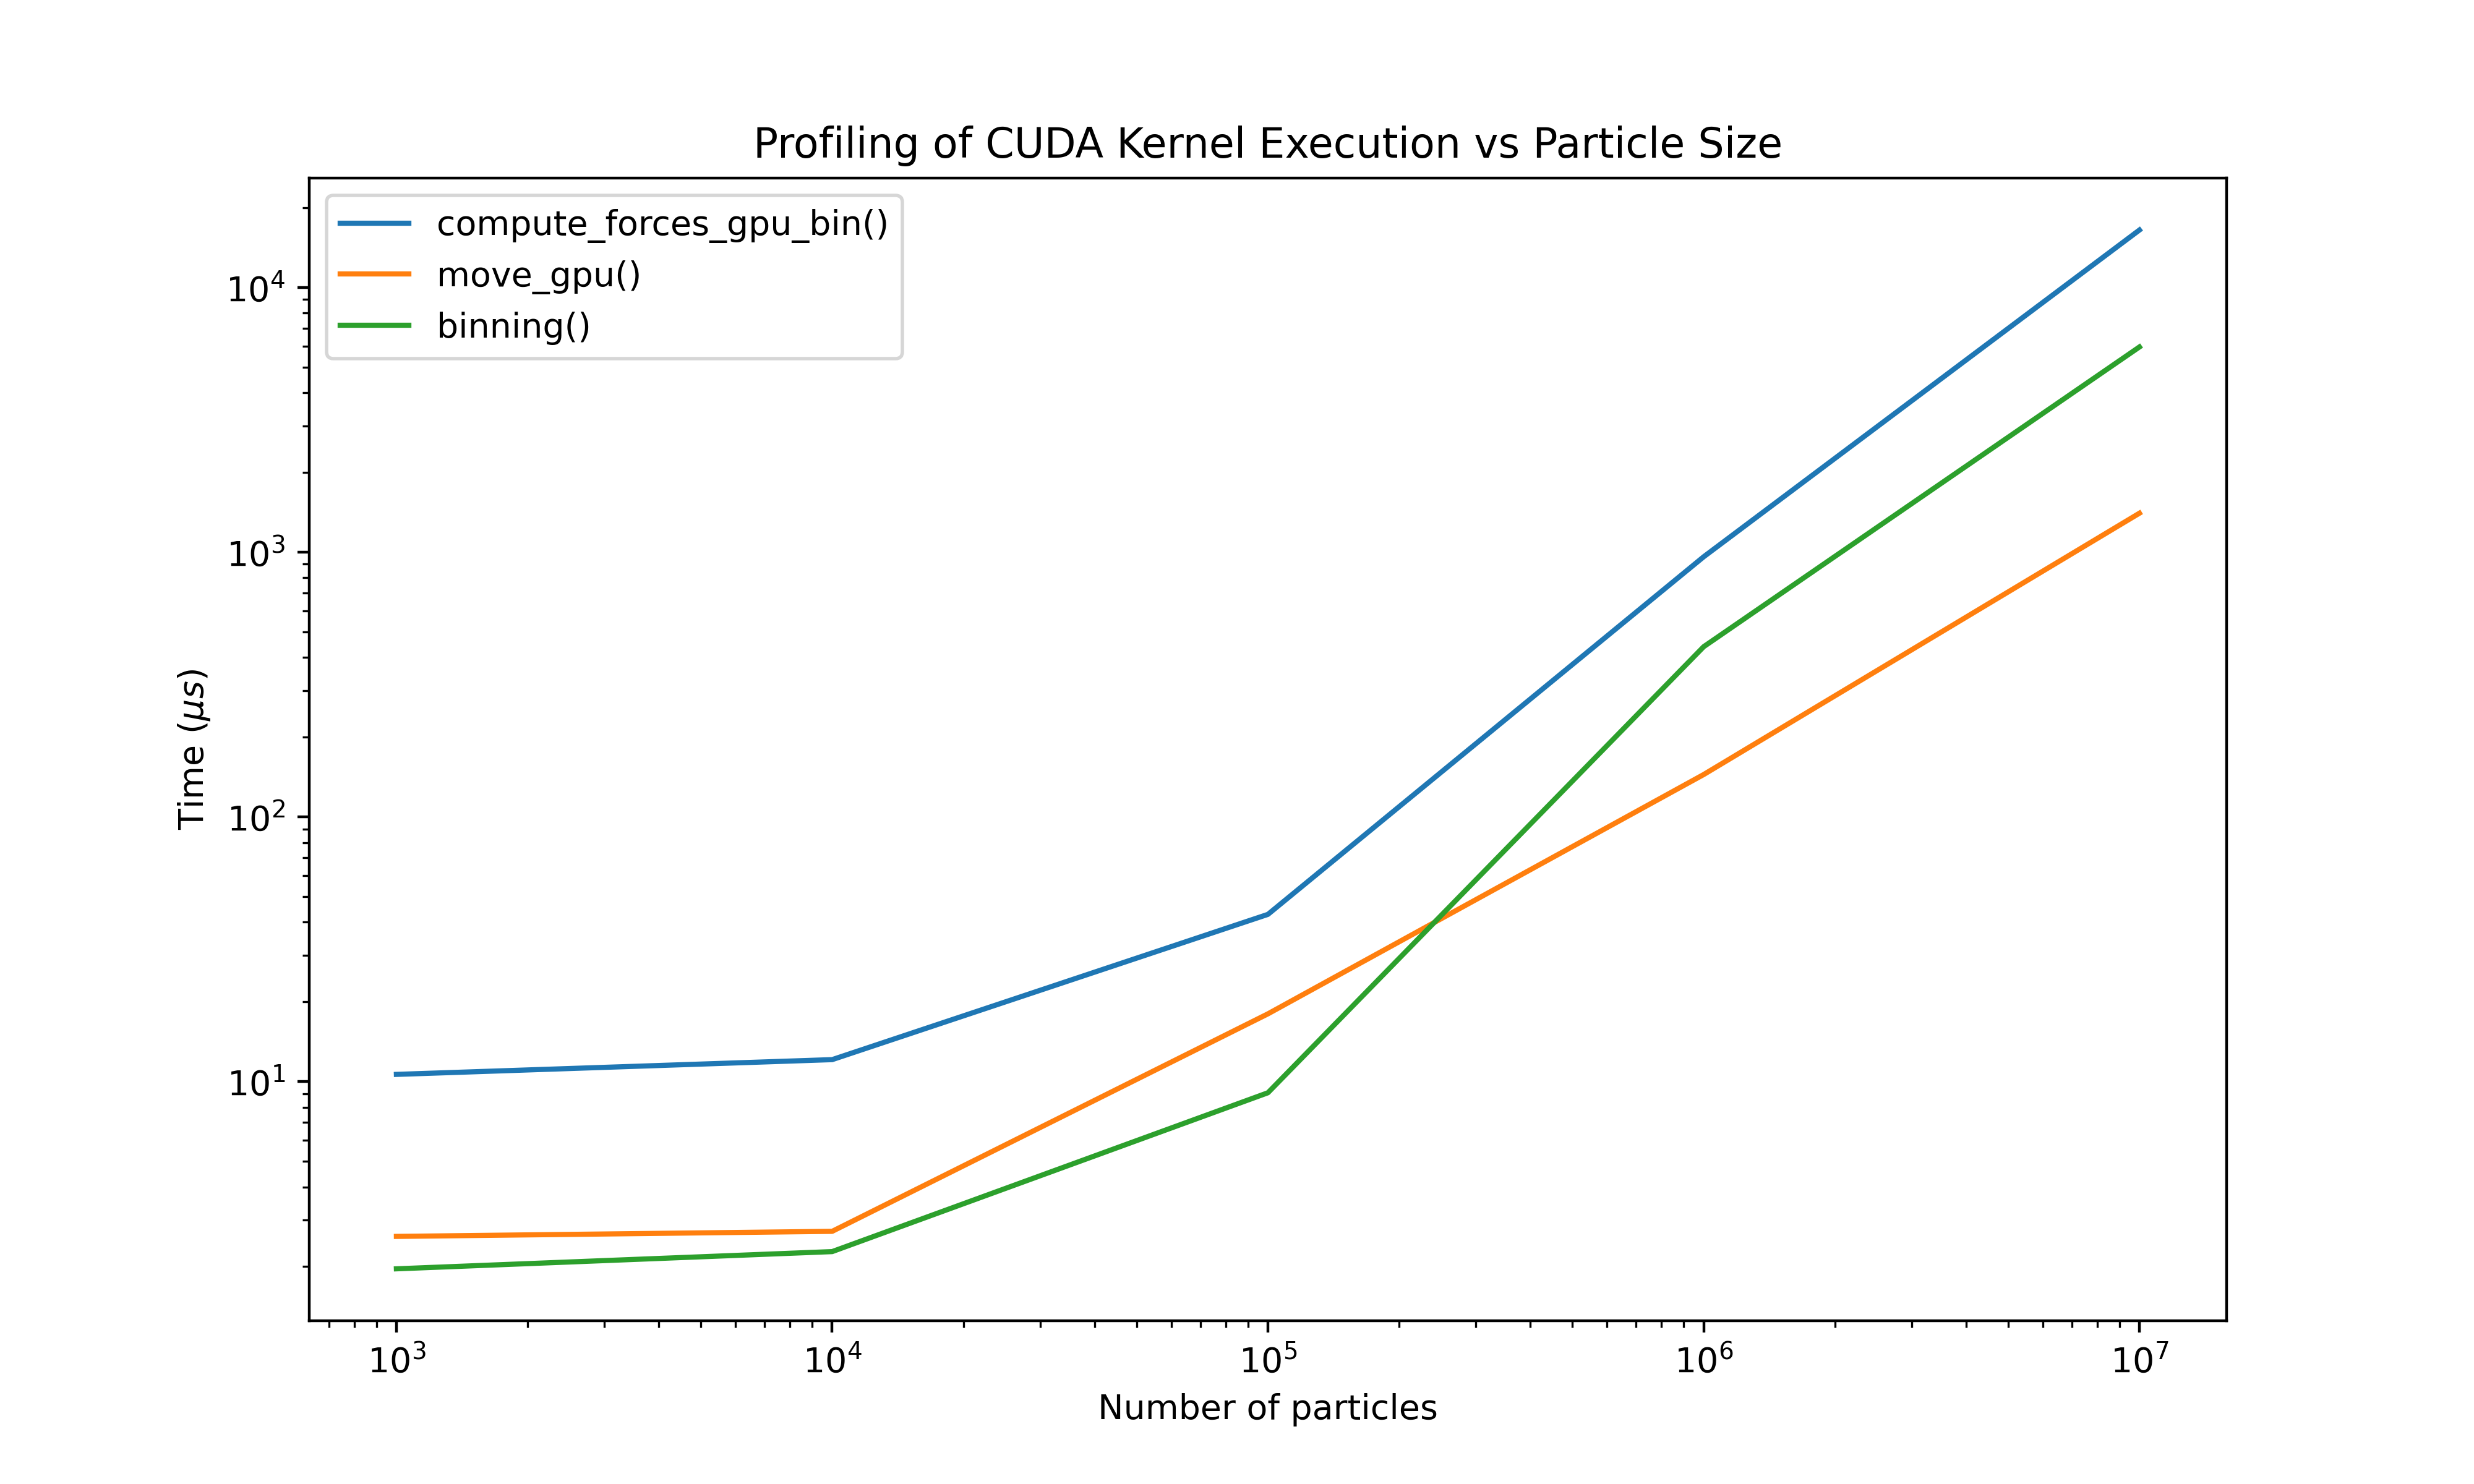
\includegraphics[width=6in]{figures/profiling.png}}

\centerline{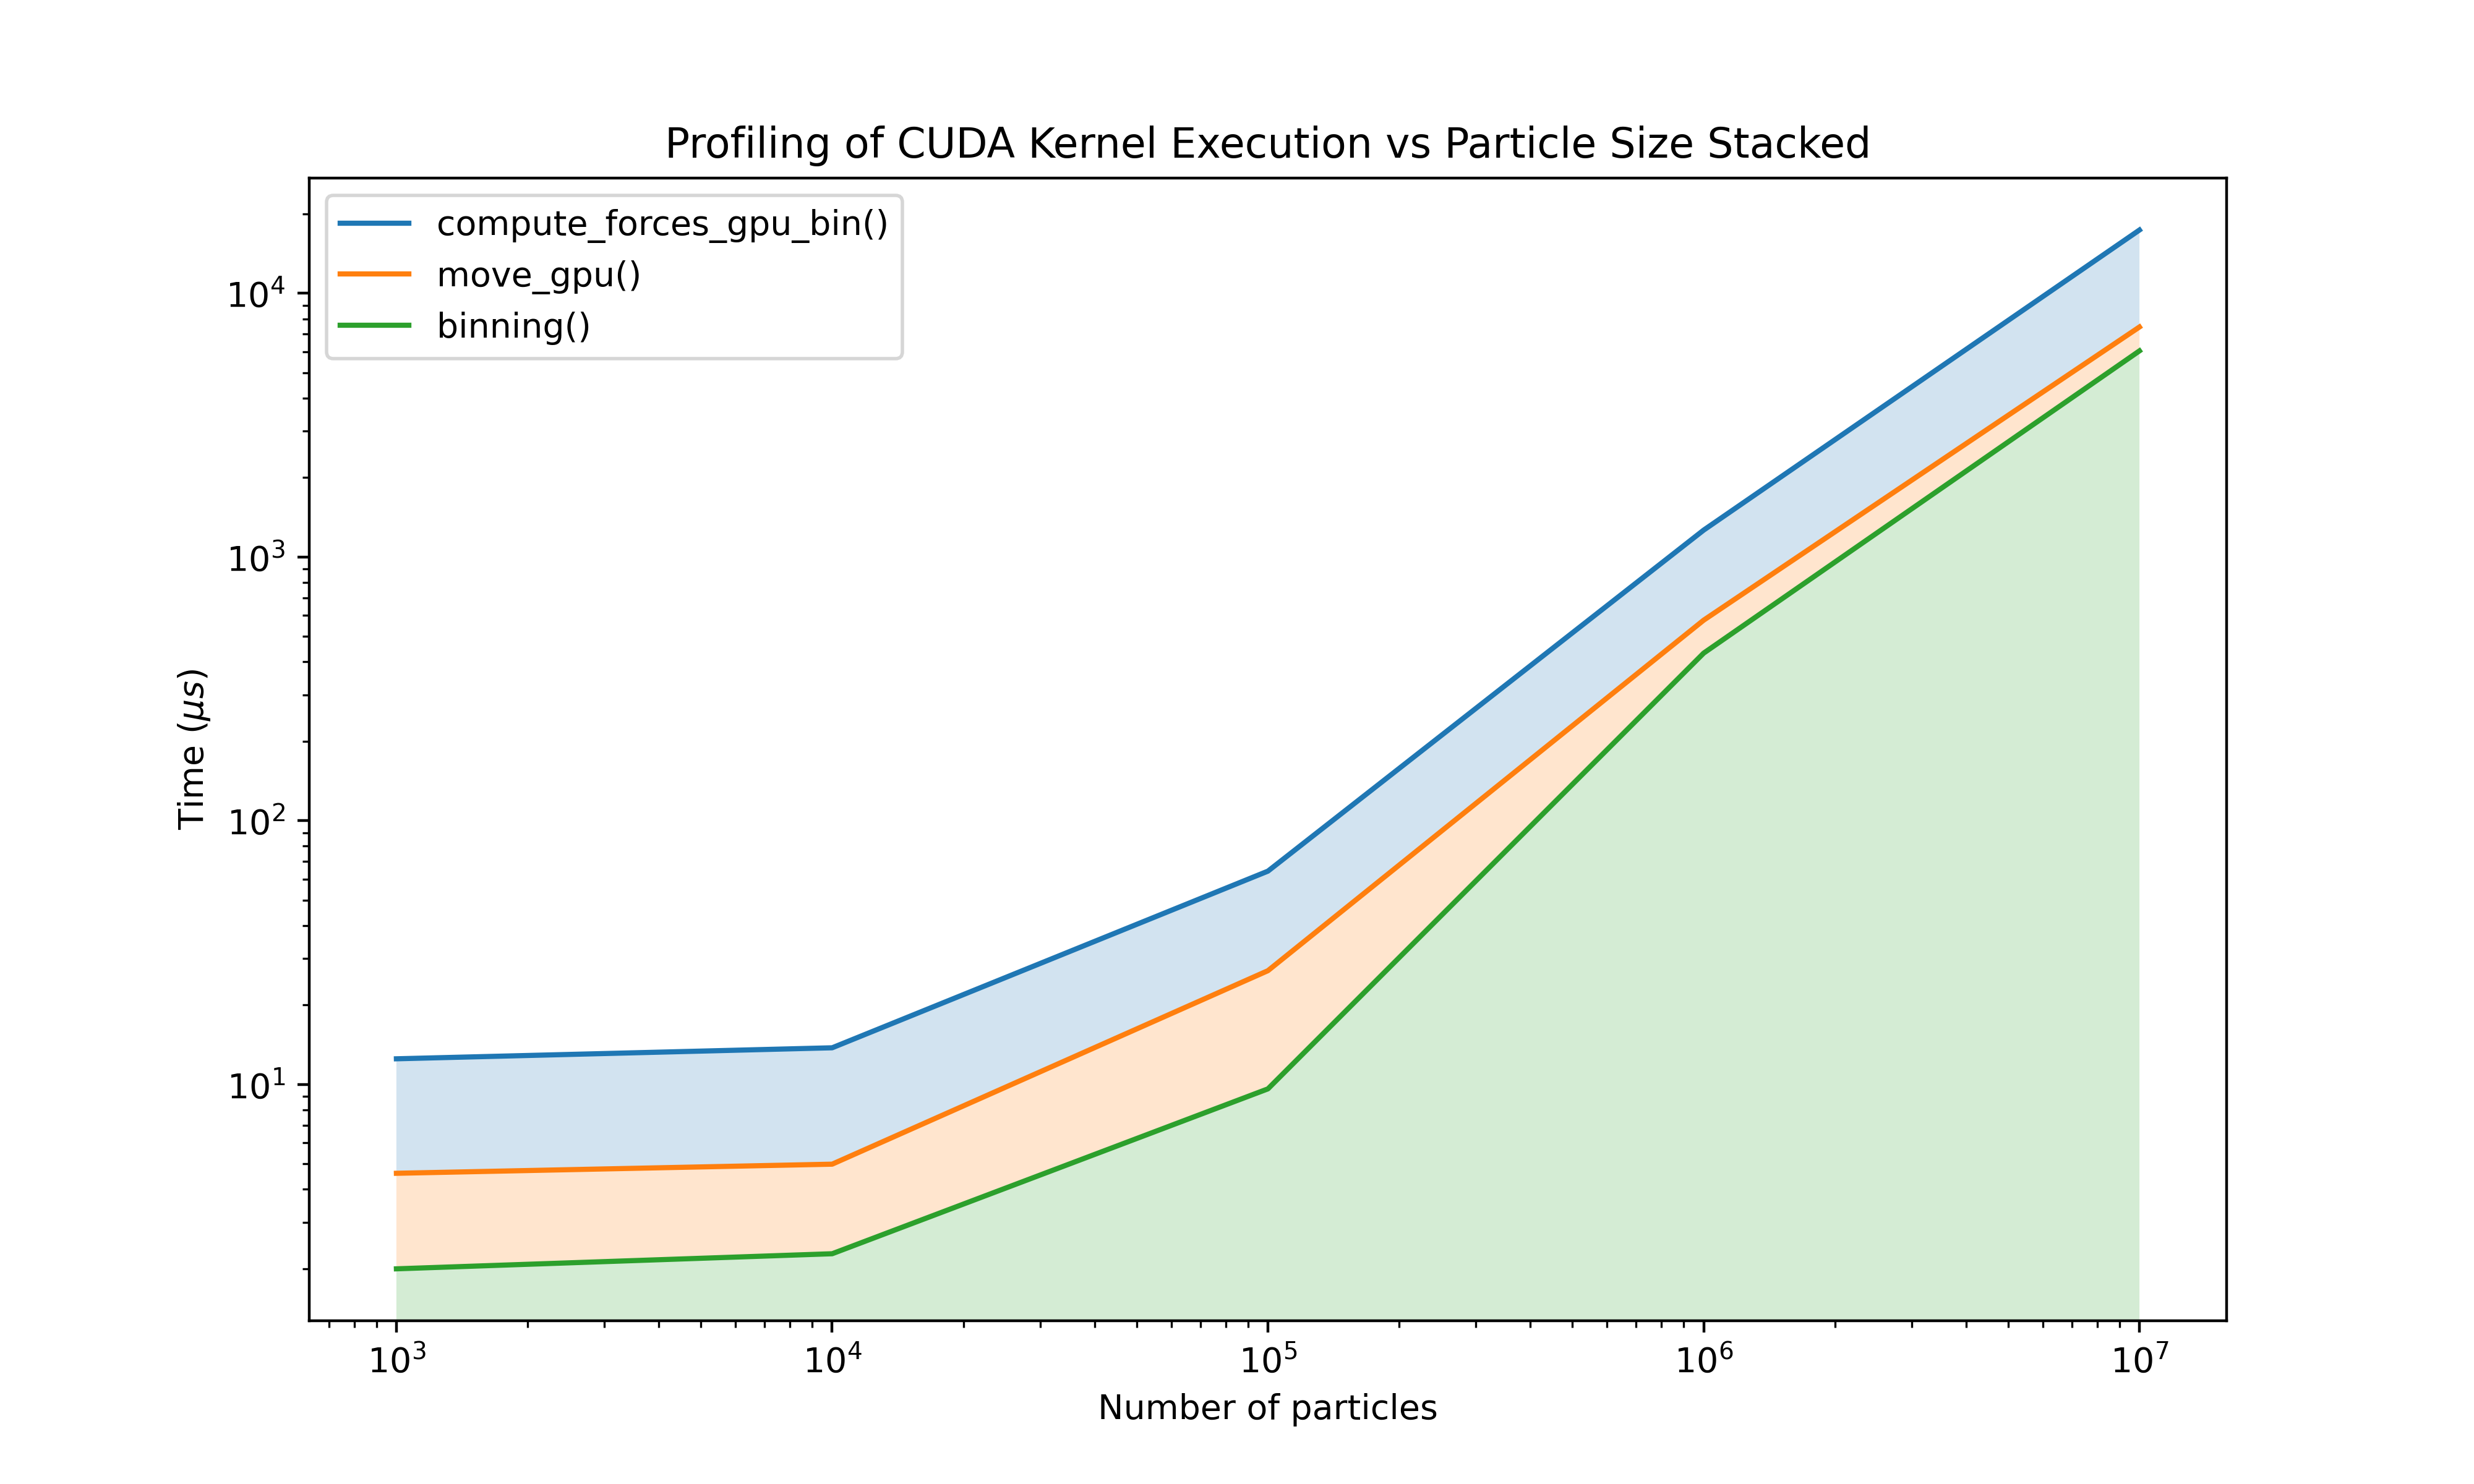
\includegraphics[width=6in]{figures/profiling-stacked.png}}

\centerline{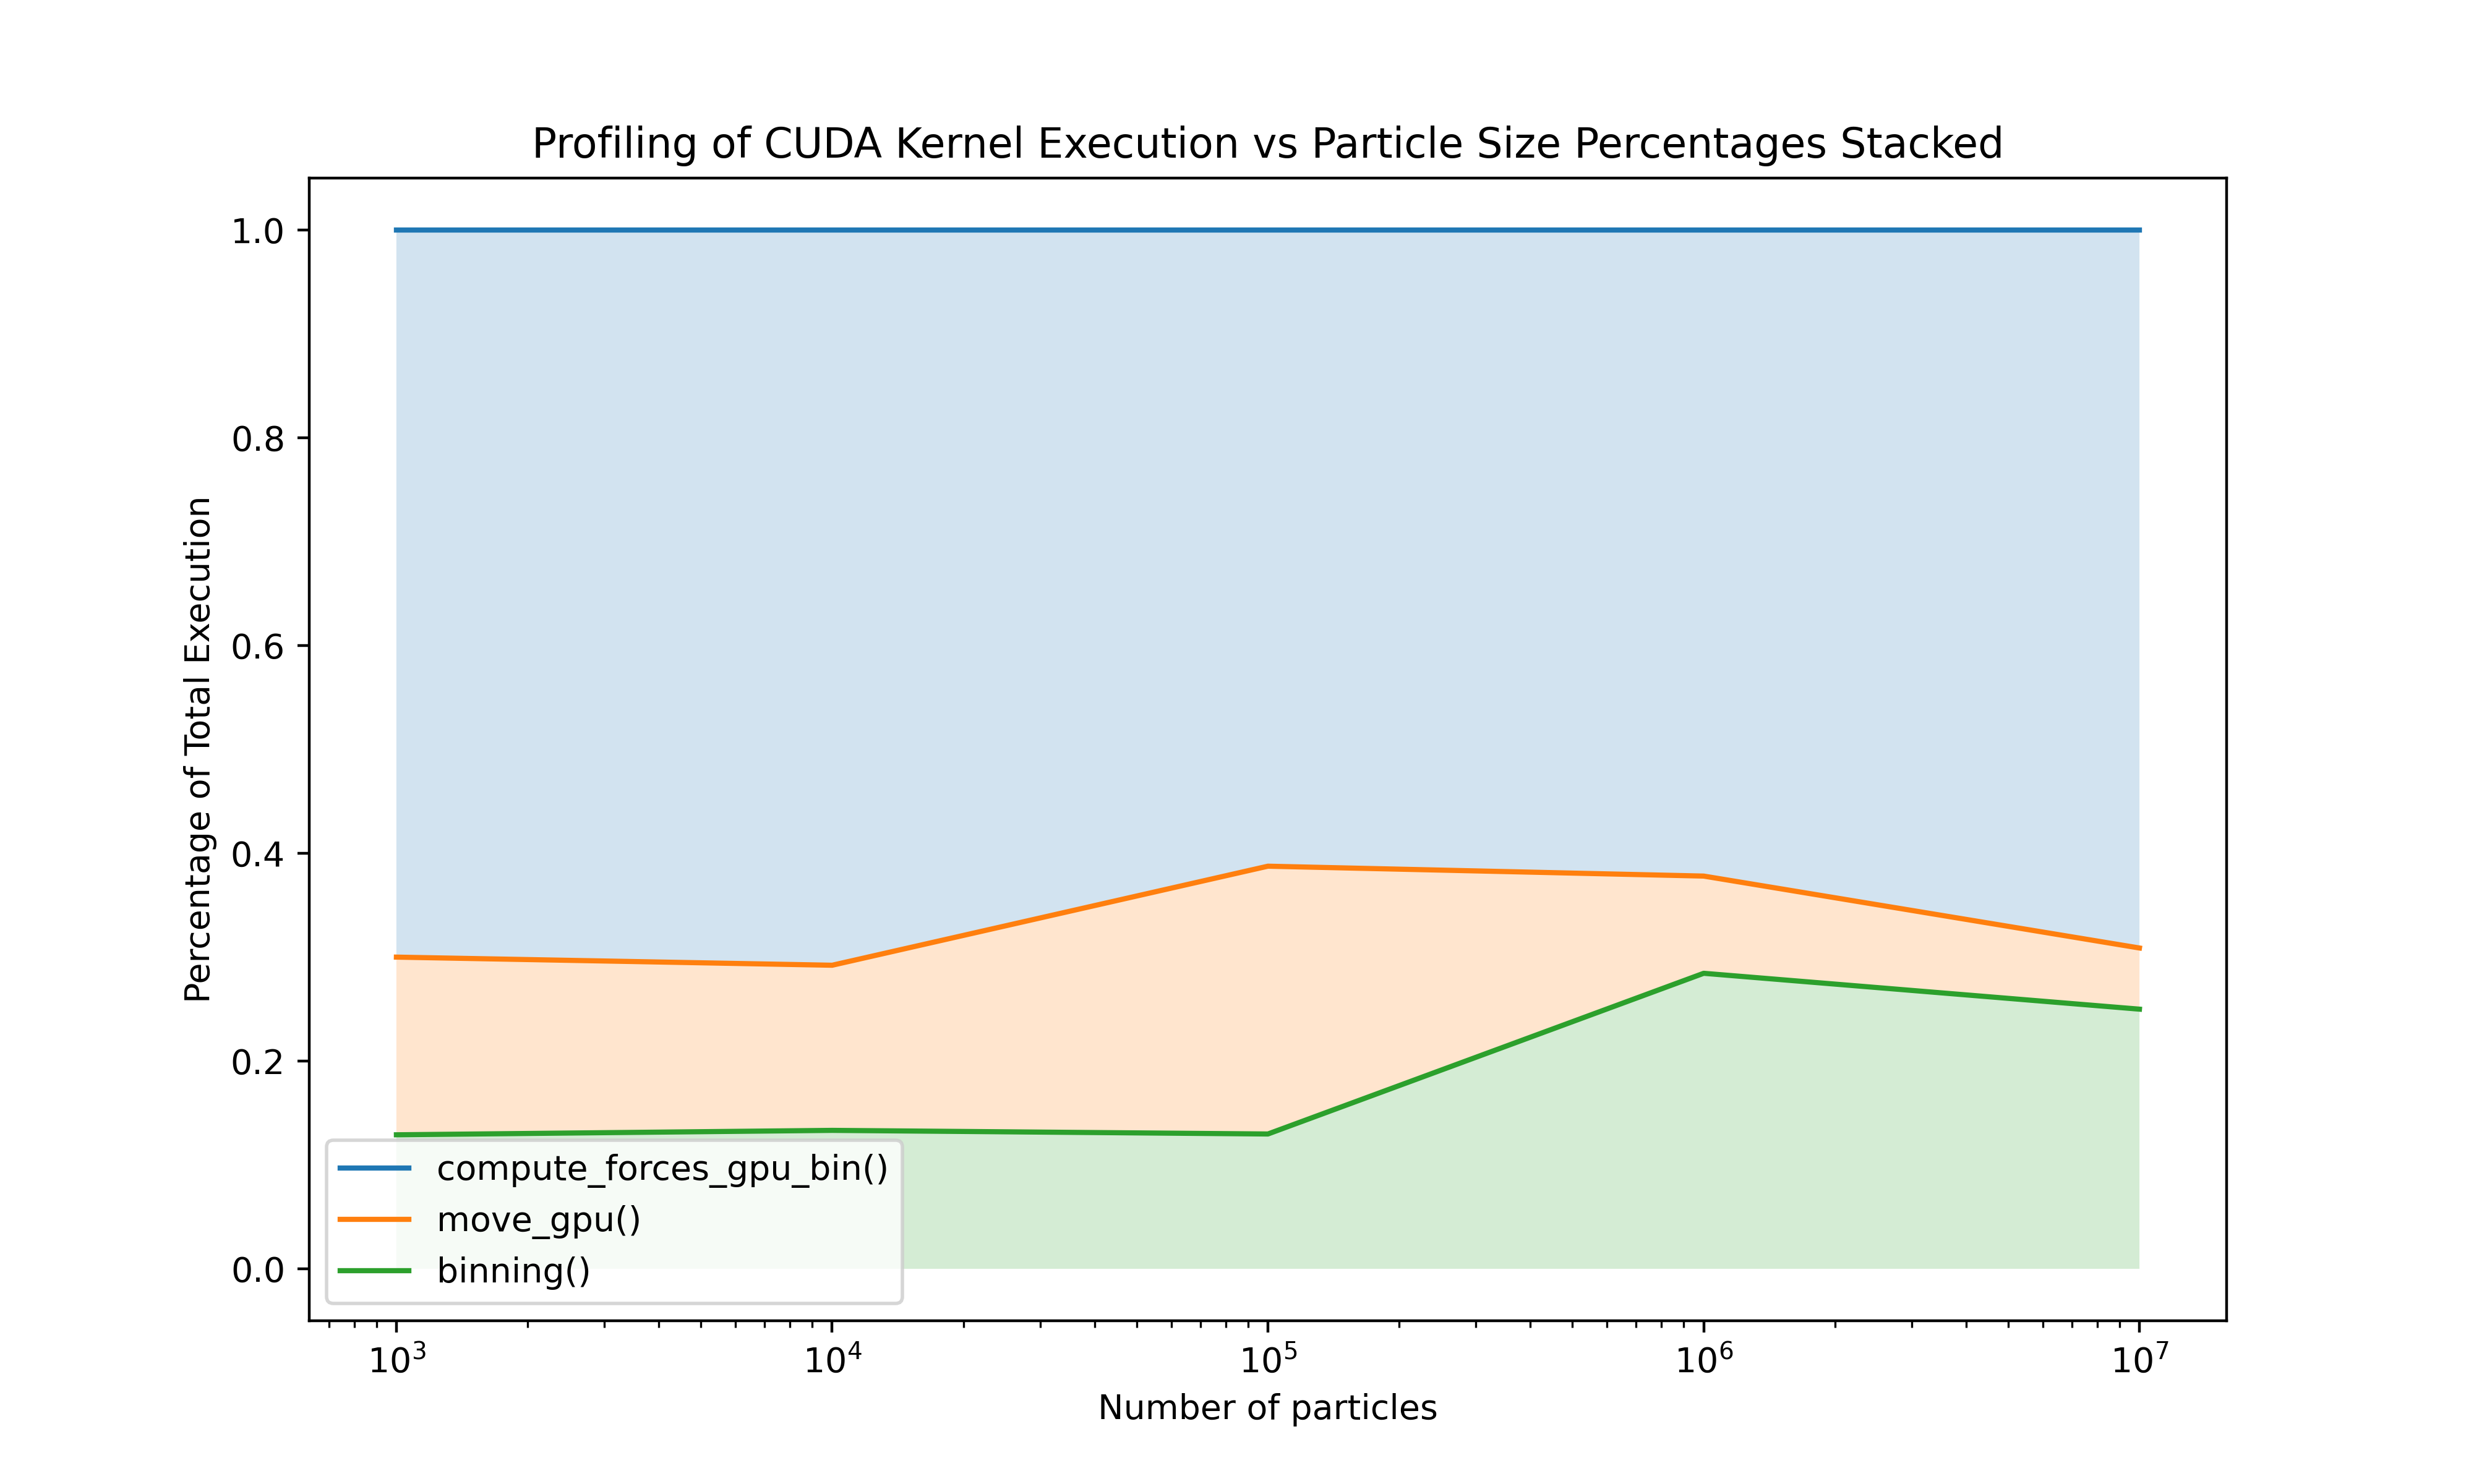
\includegraphics[width=6in]{figures/profiling-stacked-percentage.png}}


\section{Contribution}
Brian contributed to most of the code and report. Andrew helped with a few edge cases and debugging. Xuan explores the usage of cuda and helps on the report.

\end{document}

